\section{Обработка табличных данных}
\verb|Задание.| Все столбцы, содержащие минимальный элемент, заменить столбцом X.

Создано окно приложения, содержащее три элемента \verb|DataGridView| и три элемента 
\verb|Button|. Для перехвата и обработки ошибок добавлен элемент \verb|ErrorProvider|
(см. рисунок \ref{fig:dgv_form}). 

\begin{figure}[H]
    \centering
    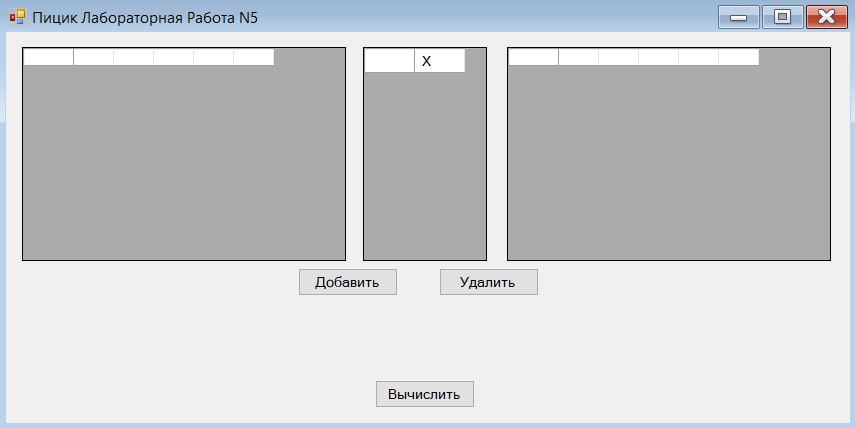
\includegraphics[scale=0.68]{../img/dgv/dgv_form.png}   
    \caption{Вид формы программы замены столбцов}
    \label{fig:dgv_form}
\end{figure}

У элементов формы изменены значения некоторых свойств, значения измененных атрибутов 
можно увидеть в таблице \ref{tab:dgv_params}.

\begin{table}[H]
    \small
    \caption{Значения атрибутов элементов формы}
    \begin{tabular}{|l|l|}\hline
    Свойство & Значение \cr\hline
    \multicolumn{2}{|l|}{Форма}\cr\hline
    \verb"Text" & Пицик Лабораторная работа N5 \cr\hline
    \multicolumn{2}{|l|}{Кнопка "Добавить"}\cr\hline
    \verb"(Name)" & btn\_add \cr\hline 
    \verb"Text" & Добавить \cr\hline 
    \multicolumn{2}{|l|}{Кнопка "Удалить"}\cr\hline
    \verb"(Name)" & btn\_rm\cr\hline
    \verb"Text" & Удалить \cr\hline
    \multicolumn{2}{|l|}{Кнопка "Вычислить"}\cr\hline
    \verb"(Name)" & btn\_calc \cr\hline 
    \verb"Text" & Вычислить \cr\hline
    \multicolumn{2}{|l|}{DataGridView для ввода}\cr\hline
    \verb"(Name)" & data\_first\cr\hline
    \verb"AllowUserToAddRows" & False\cr\hline
    \verb"AllowUserToDeleteRows" & False\cr\hline
    \multicolumn{2}{|l|}{DataGridView для столбца X}\cr\hline
    \verb"(Name)" & data\_x \cr\hline
    \verb"AllowUserToAddRows" & False\cr\hline
    \verb"AllowUserToDeleteRows" & False\cr\hline
    \multicolumn{2}{|l|}{DataGridView для вывода}\cr\hline
    \verb"(Name)" & data\_result \cr\hline
    \verb"AllowUserToAddRows" & False\cr\hline
    \verb"AllowUserToDeleteRows" & False\cr\hline
    \verb"ColumnHeadersHeightSizeMode" & AutoSize \cr\hline
    \verb"ReadOnly" & True \cr\hline
    \multicolumn{2}{|l|}{Обработчик ошибок}\cr\hline
    \verb"(Name)" & error\_prov \cr\hline
    \end{tabular}
    \label{tab:dgv_params}
\end{table}

С помощью параметров столбцов элемента \verb|DataGridView|, контекстное меню которых можно 
вызвать, нажав на стрелочку около элемента и на свойство <<Правка столбцов>>, у элемента 
\verb|data_x| было добавлено название столбца <<X>> \cite{book_msvisual}.

Для добавления столбцов, в кнопке <<Добавить>> был разработан следующий код \cite{book_tmp}:
\begin{minted}[linenos, style=bw, fontsize=\small, breaklines=true]{cpp}
private: System::Void btn_add_Click(System::Object^ sender, System::EventArgs^ e) 
  {
    data_first->Rows->Add();
    data_x->Rows->Add();
    data_result->Rows->Add();
  }
\end{minted}

Для удаления столбцов, в кнопке <<Удалить>> был разработан следующий код:
\begin{minted}[linenos, style=bw, fontsize=\small, breaklines=true]{cpp}
private: System::Void btn_rm_Click(System::Object^ sender, System::EventArgs^ e) {
  if (data_first->CurrentRow != nullptr && !data_first->CurrentRow->IsNewRow)
  {
    int rowIndex = data_first->CurrentRow->Index;

    if (rowIndex < data_first->Rows->Count)
    // удаляем строку из data_first
    data_first->Rows->RemoveAt(rowIndex);

    // проверяем есть ли rowIndex в data_x
    if (rowIndex < data_x->Rows->Count)
      // удаляем строку из data_x по тому же индексу
      data_x->Rows->RemoveAt(rowIndex);

    // проверяем есть ли rowIndex в data_result
    if (rowIndex < data_result->Rows->Count)
      // удаляем строку из data_result по тому же индексу
      data_result->Rows->RemoveAt(rowIndex);
  }
}
\end{minted}
В переменную \verb|rowIndex| записывается индекс выбранной строки \verb|DataGridView|.
Затем, для предотвращения ошибок, перед удалением строки из каждого элемента \verb|DataGridView|,
производится проверка, что индекс выбранной строки не превышает общее количество строк каждого элемента.
Затем, если условие соблюдается, осуществляется удаление строк.

Для корректного отображения ошибок, была реализована вспомогательная функция \verb|ClearAll()|:
\begin{minted}[linenos, style=bw, fontsize=\small, breaklines=true]{cpp}
void ClearAll()
{
    error_prov->SetError(btn_calc, "");
}
\end{minted}

С остальными кодами можно ознакомиться в приложении \ref{app:codes}.

При запуске приложения открывается окно(см. рисунок \ref{fig:dgv_onlaunch}).

\begin{figure}[H]
\centering
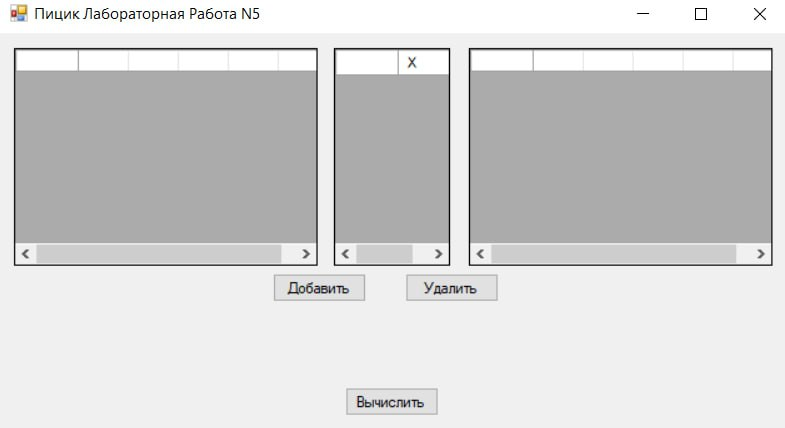
\includegraphics[scale=.65]{../img/dgv/dgv_on_launch.jpg}
\caption{<<Табличные данные>>: звпуск программы}
\label{fig:dgv_onlaunch}
\end{figure}

Ввод некорректных данных обрабатывается с помощью \verb|ErrorProvider| и сопровождается 
выводом сообщения об ошибке (см. рисунок \ref{fig:dgv_error}). 
\begin{figure}[H]
    \centering
    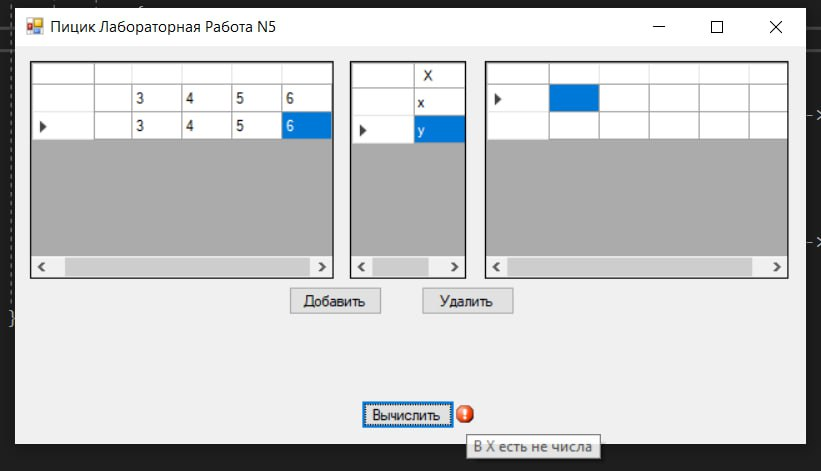
\includegraphics[scale=0.68]{../img/dgv/dgv_error.png}
    \caption{<<Табличные данные>>: сообщение об ошибке}
    \label{fig:dgv_error}
\end{figure}

Пример корректной работы программы изображен на рисунке \ref{fig:dgv_result}. 
\begin{figure}[H]
    \centering
    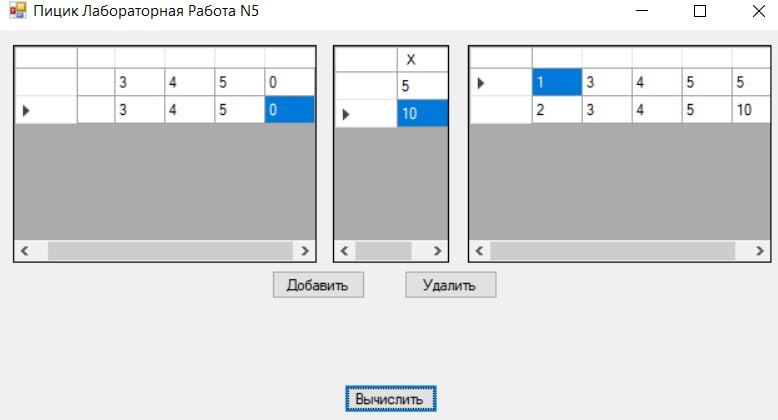
\includegraphics[scale=0.68]{../img/dgv/dgv_result.png}
    \caption{<<Табличные данные>>: работа программы}
    \label{fig:dgv_result}
\end{figure}

Полный код программы приведён в приложении \ref{app:repo}. 